% vim: set spelllang=fr foldmethod=marker:
\section{Choisir un processus de sélection}

    \subsection{Choisir un processus adapté à la situation}
Plusieurs méthodes de sélection des \cns ont été proposées, et leurs performances ont été mesurées à travers un jeu de simulations.
Il est temps désormais d'en tirer des conclusions, et de déterminer quelle méthode est préférable pour un cas d'utilisation donné.
Car il n'y a pas vraiment de «meilleure méthode» adaptable à toutes les applications, chacune possède ses avantages et ses inconvénients.

\paragraph{Aucun renouvellement des \cns}
Ne pas renouveler les \cns permet de garder en vie très longtemps les nœuds qui ne sont pas sélectionnés, mais n'assure que très mal la sécurité du réseau.
Les \cns d'origine vont rapidement épuiser leur batterie et tomber hors service.
De plus, si la sélection est réalisée de telle sorte que tous les capteurs du cluster ne soient pas couvert par un \cn\,\footnote{Ou même, en réalité, par le nombre minimal de \cns nécessaire pour reporter effectivement une attaque, puisque par principe le \ch attend de recevoir des alarmes de la part de plusieurs \cns distincts avant de déclarer un capteur comme compromis, ceci afin d'éviter les faux positifs (accidentels ou d'origine malveillante).}, alors certains nœuds ne seront jamais surveillés.
La mise en place des \cns sans renouvellement n'est donc pas conseillée, en dehors de cas particuliers où les \cns sont connus d'avance, disposent de composants matériels distincts des autres capteurs (une meilleure batterie, notamment), et sont expressément disposés de manière à assurer une couverture suffisante du cluster.

\paragraph{Renouvellement périodique: sélection pseudo-aléatoire}
Le processus de renouvellement des \cns par sélection aléatoire est un excellent compromis entre sécurité et longévité du réseau: cette méthode, simple à mettre en place, ne requiert que peu d'échanges de données de contrôle, et consomme peu d'énergie (en dehors du surcout inévitable induit par l'usage des \cns).
Lorsque les premiers nœuds épuisent leur batterie, le nombre moyen de \cns élus s'adapte, puisqu'il s'agit d'un pourcentage souhaité sur les nœuds en activité, et non d'un nombre prédéfini fixe.
L'équilibre en termes de consommation énergétique ne sera pas aussi bon qu'avec d'autres méthodes: l'application ne doit pas craindre de perdre certains capteurs avant les autres.
De même, le niveau de sécurité n'est pas à son maximum, puisque certains capteurs peuvent se retrouver en dehors du champ de couverture des \cns pour une phase donnée.
Cependant, le renouvellement fréquent et les lois des probabilités font qu'un nœud compromis devrait être rapidement détecté, au plus au bout de quelques phases successives.

\paragraph{Renouvellement périodique: sélection selon l'énergie résiduelle}
L'utilisation des \vns permet de sécuriser le processus de renouvellement selon l'énergie résiduelle, mais au prix d'un cout très important en énergie.
La répartition de la charge sur les capteurs du cluster est excellente, mais ne dépasse pas celle obtenue par la méthode d'élection démocratique, qui consomme moins d'une manière générale, une fois sa phase initiale amortie.
Le seul cas d'usage pour cette méthode serait éventuellement un réseau pour lequel l'équilibre en énergie résiduelle des capteurs est important, mais qui ne connaitrait que de faibles périodes d'activités, par exemple si tous les capteurs s'allument sur une durée de quelques minutes, effectuent des mesures, puis s'éteignent pour plusieurs heures.
Dans les autres cas, le processus d'élection démocratique lui sera préféré.

\paragraph{Renouvellement périodique: élection démocratique}
Les performances du processus d'élection démocratique sont similaires à celles de la méthodes selon l'énergie résiduelle pour ce qui est de l'équilibre de la charge dans le cluster, \cad qu'elles sont excellentes.
La consommation générale en énergie est meilleure, une fois la période initiale «amortie», mais elle est loin d'égaler celle de la méthode de sélection aléatoire.
La contrainte imposée de couvrir chaque capteur par au moins deux \cns assure un bon niveau de surveillance, et la sécurité du dispositif est garantie par les «votes» des \cns qui aident le \ch à désigner leurs successeurs.
Cette méthode possède un autre avantage: en réutilisant la surveillance effectuée par les \cns lorsque vient le moment de renouveler la sélection, il est possible d'utiliser d'autres facteurs pour choisir les nœuds, comme la puissance des signaux émis, l'index de connectivité des capteurs, ou encore leur indice de \idx{confiance}.
Cette méthode est utilisable pour des applications qui ont des contraintes fortes en termes d'équilibre de la consommation, \cad des applications qui doivent conserver l'ensemble des capteurs en fonctionnement le plus longtemps possible.

Les avantages et inconvénients de chaque méthode sont résumés en \tabref{sd:table:strweak}.
La \tabref{sd:table:apps}, quant à elle, synthétise les cas d'utilisation de ces processus.
\begin{table}[ht]
    \centering
    \caption{Avantages et inconvénients des différents processus de sélection}\label{sd:table:strweak}
    \medskip
    \small
    \begin{tabu}{X[1,c,m] X[2,j,m] X[2,j,m]}
        \toprule
        \textsc{Méthode} & \textsc{Avantages} & \textsc{Inconvénients} \\
        \midrule
        Aucun\newline renouvellement
            & \textbullet\;Préservation des nœuds non sélectionnés
            & \textbullet\;Mauvaise surveillance
            \\
        \midrule
        Sélection aléatoire
            & \textbullet\;Consommation d'énergie modérée\newline
              \textbullet\;Simple à mettre en œuvre\newline
              \textbullet\;Le nombre de \cns sélectionnés est statistiquement un pourcentage constant sur le nombre de capteurs en activité\newline
              \textbullet\;Bonne rotation des \cns; processus aléatoire, donc pas d'attaques
            & \textbullet\;Équilibre moyen de la consommation en énergie dans le cluster\newline
              \textbullet\;Risque d'avoir des capteurs non couverts par les \cns lors de certaines phases
            \\
        \midrule
        Sélection selon l'énergie résiduelle
            & \textbullet\;Bonne répartition de l'équilibre\newline
              \textbullet\;Surveillance de tous les capteurs par au moins deux \cns
            & \textbullet\;L'ajout de \vns est contraignant; couteux en énergie et lourd à implémenter\newline
              \textbullet\;Très gourmand en énergie
            \\
        \midrule
        Élection démocratique
            & \textbullet\;Bonne répartition de l'équilibre\newline
              \textbullet\;Surveillance de tous les capteurs par au moins deux \cns\newline
              \textbullet\;Consommation d'énergie modérée (après la période initiale)\newline
              \textbullet\;Adaptation possible pour prendre en compte d'autres paramètres
            & \textbullet\;La période initiale consomme beaucoup d'énergie
            \\
        \bottomrule
    \end{tabu}
\end{table}
\begin{table}[ht]
    \centering
    \caption{Cas d'utilisation proposés pour les différentes méthodes de sélection}\label{sd:table:apps}
    \medskip
    \small
    \begin{tabu}{X[1,c,m] X[2,j,m]}
        \toprule
        \textsc{Méthode} & \textsc{Cas d'utilisation} \\
        \midrule
        Aucun renouvellement
            & Fortement déconseillé de manière générale (la sécurité apportée ne vaut pas de mettre en place le dispositif, sauf en cas d'usage de capteurs dédiés du point de vue matériel)
            \\
        \midrule
        Sélection aléatoire
            & Applications dont la sécurité n'est pas une priorité absolue, dont on veut garder des capteurs en vie très longtemps (mais pas nécessairement \emph{tous} les capteurs).
            \\
        \midrule
        Sélection selon l'énergie résiduelle
        & \textit{A~priori}, mieux vaut utiliser l'élection démocratique; sauf en cas de courtes périodes d'activité du cluster.
            \\
        \midrule
        Élection démocratique
            & Applications dont la sécurité est essentielle, et dont il faut maintenir en activité la totalité des capteurs. Déconseillée pour des applications imposant de courtes périodes d'activité au cluster.
            \\
        \bottomrule
    \end{tabu}
\end{table}

    \subsection{Adapter le processus au réseau}

        \subsubsection{Nombre des \cns}
Les résultats numériques de la section précédente, et notamment les différences de performances sur l'usage du processus d'élection démocratique pour désigner sept~ou dix~nœuds mettent en évidence l'importance du nombre de \cns dans le cluster sur la préservation de l'énergie.
Comme les \cns consomment davantage, plus ils sont nombreux, plus les réserves se vident rapidement; mais plus les chances de détecter l'attaque sont élevées.
Il est donc intéressant, lors du déploiement du réseau, d'observer quel est le nombre idéal de \cns à sélectionner pour assurer une couverture correcte sans gaspiller trop d'énergie.
Dans notre cas, descendre à sept~\cns semble raisonnable, surtout avec des méthodes qui assurent une couverture minimale.
En dessous de cette valeur, le risque de laisser des zones non couvertes devient important.

Le nombre de \cns à utiliser est très dépendant de la topologie du réseau.
Pour rappel, nous avons travaillé jusqu'à maintenant dans un cluster dont tous les nœuds sont des voisins directs du \ch.
Si les \cns sont appelés à être déployés sur une autre architecture, sans cluster par exemple, les problèmes de couverture seront différents.

        \subsubsection{Contraintes sur la couverture du cluster}
Un exemple déjà abordé dans le chapitre précédent est celui d'un réseau en étoile, comme présenté en \figref{sd:fig:star}: dans une telle configuration, il est indispensable d'adapter (ou de supprimer) la règle selon laquelle chaque capteur doit être surveillé par au moins deux~\cns (pour les méthodes d'élection démocratique et de sélection selon l'énergie résiduelle), sans quoi tous les nœuds ou presque devront être sélectionnés en tant que \cns.
\begin{figure}[!ht]
    \centering
    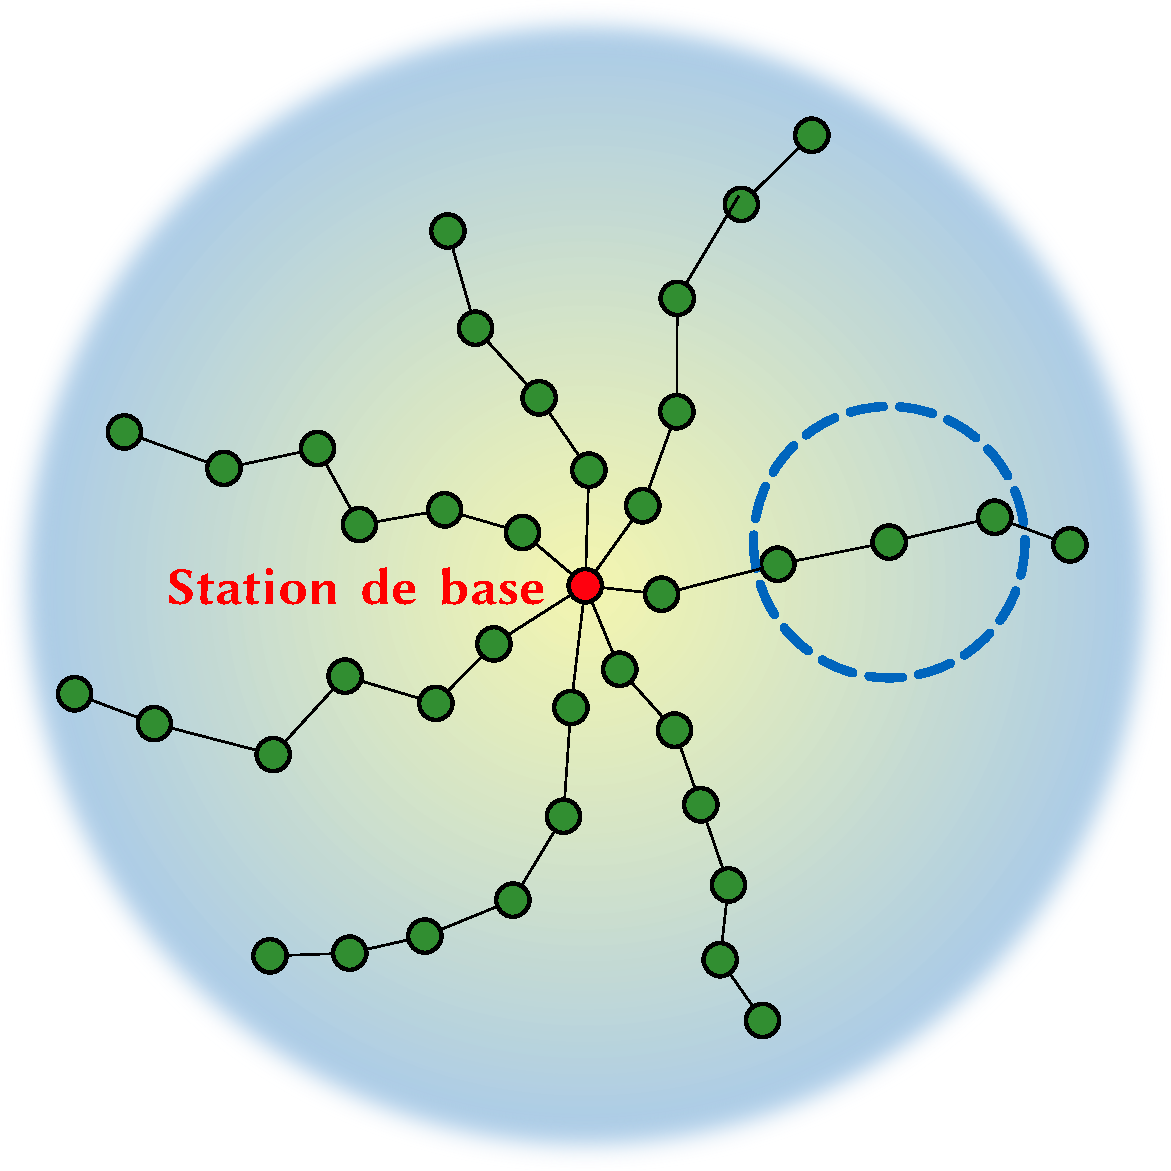
\includegraphics[width=7cm]{\chapterfig/WSN_star.pdf}
    \caption[Schéma d'un réseau de capteurs en forme d'étoile]{Schéma d'un réseau de capteurs en forme d'étoile. Le cercle en pointillés bleus représente la portée d'un nœud.}\label{sd:fig:star}
\end{figure}
Pour autant, cette règle n'est pas à rejeter systématiquement: elle est très utile dans la configuration avec cluster que nous avons étudié, et permet d'y limiter le nombre de \cns à désigner.

        \subsubsection{Interactions entre \cns et nœuds compromis}
La mise en place d'un système de détection efficace passe également par une implémentation rigoureuse de l'algorithme utilisé par les \cns pour détecter les attaques.
Aucune recommandation particulière n'est fournie, si ce n'est de définir en amont du déploiement un cahier des charges précis couvrant les cas d'utilisation et de fonctionnement normaux du réseau, de manière à pouvoir mettre en œuvre les règles de détection de la façon la plus efficace possible.

Conjugué à un renouvellement périodique selon une méthode de détection aléatoire ou d'élection démocratique, l'usage des \cns permet une surveillance efficace du réseau.
Il serait tout de même appréciable de pouvoir construire un modèle plus formel de cette surveillance.
Puisque nous avons plusieurs acteurs avec des buts différents, les capteurs «sains» et les nœuds compromis, c'est vers des éléments de la théorie des jeux que nous allons nous tourner.
